
%\renewcommand{\theequation}{\theenumi}
%\begin{enumerate}[label=\arabic*.,ref=\thesubsection.\theenumi]
%\numberwithin{equation}{enumi}

\item A=$[a_{ij}]_{mxn}$ is a square matrix,if\\
(A) m$<$n (B)m$>$n (C) m=n (D) None of these\\
\item Which of the given values of x and y make the following pair of matrices equal \myvec{3x+7 &5\\y+1 &2-3x},\myvec{0 &y-2\\8 &4}\\
(A)x=$\frac{-1}{3}$,y=7 \\
 (B) Not possible to find\\
(C) y=7, x=$\frac{-2}{3}$\\
 (D) x=$\frac{-1}{3}$,y=$\frac{-2}{3}$\\
\item The number of all possible matrices of order 3X3 with each entry 0 or 1 is:\\
(A) 27 (B)18 (C)81 (D)512\\
\item Let A=\myvec{2 &4\\3 &2},B=\myvec{1 &3\\-2 &5},C=\myvec{-2 &5\\3 &4}
Find each of the following:\\
(i) A+B  (ii)A-B  (iii)3A-C  (iv)AB  (v)BA\\
\item Compute the following:\\
(i)\myvec{a &b\\-b &a}+\myvec{a &b\\b&a} (ii)\myvec{a^2+b^2 &b^2+c^2\\a^2+c^2 &a^2+b^2}+\myvec{2ab &2bc\\-2ac &-2ab} \\
  (iii) \myvec{-1 &4 &-6\\8 &5 &16\\2 &8 &5}+\myvec{12 &7 &6\\8 &0 &5\\3 &2 &4}\\ 
(iv) \myvec{cos^2x &sin^2x\\sin^2x &cos^2x}+\myvec{sin^2x &cos^2x\\cos^2x &sin^2x}\\
\item Compute the indicated products.
\begin{enumerate}
\item \myvec{2 &3 &4\\3 &4 &5\\4 &5 &6}\myvec{1 &-3 &5\\0 &2 &4\\3 &0 &5} 
\item \myvec{2 &1\\3 &2\\-1 &1}\myvec{1 &0 &1\\-1 &2 &1} \\
\item  \myvec{3 &-1 &3\\-1 &0 &2}\myvec{2 &-3\\1 &0\\3 &1}
\end{enumerate}
\item If,A=\myvec{1 &2 &-3\\5 &0 &2\\1 &-1 &1},B=\myvec{3 &-1 &2\\4 &2 &5\\2 &0 &3}and C=\myvec{4 &1 &2\\0 &3 &2\\1 &-2 &3},then compute (A+B) and (B-C).Also ,verify that A+(B-C)=(A+B)-C.\\
\item If A=$\myvec{\frac{2}{3} & 1 & \frac{5}{3}\\ \frac{1}{3} & \frac{2}{3} & \frac{4}{3} \\ \frac{7}{3} &2  & \frac{2}{3}}$ and B=$\myvec{\frac{2}{5} & \frac{3}{5} &1 \\ \frac{1}{5} & \frac{2}{5} & \frac{4}{5}\\ \frac{7}{5} & \frac{6}{5} & \frac{2}{5}}$,then compute 3A-5B.\\

\item Find x and y,if 2 \myvec{1 &3\\0 &x}+\myvec{y &0\\1 &2}=\myvec{5 &6\\1 &8}\\
\item Solve the equation for x,y,z and t,if \\
2\myvec{x &z\\y &t}+3\myvec{1 &-1\\0 &2}=3\myvec{3 &5\\4 &6}\\
\item If x=\myvec{2 \\3}+y\myvec{-1 \\1}=\myvec{10 \\5},find the values of x and y.\\
\item Given 3\myvec{x &y\\z &w}=\myvec{x &6\\-1 &2w}+\myvec{4 &x+y\\z+w &3},find the values of x,y,z and w.\\


\item The bookshop of a particular school has 10 dozen chemistry books, 8 dozen
physics books, 10 dozen economics books. Their selling prices are \rupee{80}, \rupee{60} and
 \rupee{40} each respectively. Find the total amount the bookshop will receive from
selling all the books using matrix algebra.\\
\solution
The total books in the bookshop can be expressed as 
\begin{align}
    \vec{A} = 12 \myvec{10 \\ 8 \\ 10}
\end{align}
and their selling price as
%
\begin{align}
    \vec{B} = \myvec{80 \\ 60 \\ 40}.
\end{align}
The total amount received by the bookshop after selling the books is given by,
\begin{align}
    \vec{A}^{\top}\vec{B} = 12 \myvec{10 & 8 & 10}\myvec{80 \\ 60 \\ 40}
    =20160
\end{align}
Assume X,Y,Z,W and P are matrices of orders $2\times n$,$3 \times k$,$2\times p$,$n\times 3$ and $p\times k$,respectively.\\
Choose the correct answer in Exercise 31 and 32.\\
\item The restriction on n,k and p so that PY+WY will be defined are:\\
(A)k=3,p=n\\
 (B)k is arbitrary,p=2 \\
 (C)p is arbitrary,k=3 \\
 (D)k=2,p=3\\
\item If n=p,then the order of the matrix 7X-5Z is:\\
(A)$p \times 2$ (B)$2 \times n$ (C)$n \times 3$ (D)$p \times n$\\
\item Find the transpose of each of the following matrices:\\
(i)\myvec{5\\ \frac{1}{2} \\-1}\\ (ii)\myvec{1 &-1\\2 &3}\\ (iii)\myvec{-1 &5 &6\\\sqrt{3} &5 &6\\2 &3 &-1}\\
\item If A=\myvec{-1 &2 &3\\5 &7 &9\\-1 &1 &1} and B=\myvec{-4 &1 &-5\\1 &2 &0\\1 &3 &1},then verify that\\
(i)$(A+B)^{'}=A^{'}+B^{'}$ \\(ii) $(A-B)^{'}=A^{'}-B^{'}$\\
\item If $A^{'}$=\myvec{3 &4\\-1 &2\\0 &1} and B=\myvec{-1 &2 &1\\1 &2 &3},then verify that\\
(i) $(A+B)^{'}=A^{'}+B^{'}$ (ii)$(A-B)^{'}=A^{'}-B^{'}$
\item If$ A^{'}$=\myvec{-2 &3\\1 &2} and B=\myvec{-1 &0\\1 &2},then find that $(A+2B)^{'}$\\

  \item (i) Show that the matrix A=\myvec{1 &-1&5\\-1 &2 &1\\5 &1 &3} is a symmetric matrix.\\
  (ii) Show that the matrix A=\myvec{0 & 1 &-1\\-1 &0 &1\\1&-1 &0} is a skew symmetric matrix.\\
  \item For the matrix A=\myvec{1 &5\\6 &7},verify that\\
  (i)$(A+A^{'})$ is a symmetric matrix\\
  (ii)$(A-A^{'})$ is a skew symmetric matrix\\
  
  \item Find $\frac{1}{2}(A+A^{'}) $and $\frac{1}{2}(A-A^{'})$,when A=\myvec{0 &a &b\\-a &0 &c\\-b &-c &0}\\
  \item Express the following matrices as the sum of a symmetric and a skew symmetric matrix:\\
  (i) \myvec{3 &5\\1 &1} \\(ii) \myvec{6 &-2 &2\\-2 &3 &-1\\2 &-1 &3} \\
  (iii) \myvec{3 &3 &-1\\-2 &-2 &1\\-4 &-5 &2}\\ (iv) \myvec{1 &5\\-1 &2}\\
  
  Choose the correct answer in question number 43 and 44\\
  \item If A,B are symmetric matrices of same order,then AB-BA is a\\
  (A)Skew symmetric matrix \\(B)Symmetric matrix\\
  (C)Zero matrix \\ (D)Identity matrix\\
  
  Using elementary transforamtions,find the inverse of each of the matrices,if it exists questions 45-61\\
  
  \item\myvec{1 &-1\\2 &3}\\
  \solution
  Let,
\begin{align}
 \vec P &=\vec{X};
\end{align}
 so,
 \begin{align}
 \vec{(PA)}^2&=\norm{\vec P-\vec A}^2\\
 &=\norm{\vec X-\vec A}^2\\
 &=\norm{\vec X}^2+\norm{\vec A}^2-2\vec X^T\vec A\label{vec/25/eq1}
 \end{align}
 and
 \begin{align}
 \vec{(PB)}^2&=\norm{\vec P-\vec B}^2\\
 &=\norm{\vec X-\vec B}^2\\
 &=\norm{\vec X}^2+\norm{\vec B}^2-2\vec X^T\vec B\label{vec/25/eq2}
 \end{align}
 The given equation is
\begin{align}
 \vec{(PA)}^2+ \vec{(PB)}^2 =2k^2\label{vec/25/eq3}
 \end{align}
 Sub \eqref{vec/25/eq1} and \eqref{vec/25/eq2}   values in \eqref{vec/25/eq3} 
\begin{align}
\norm{\vec X}^2+\norm{\vec A}^2-2\vec X^T\vec A+\norm{\vec X}^2+\norm{\vec B}^2-2\vec X^T\vec B=2k^2\\
\implies 2\norm{\vec X}^2+\norm{\vec A}^2+\norm{\vec B}^2-2\vec X^T(\vec A+\vec B)=2k^2\label{vec/25/eq4} 
\end{align}
sub $\vec A$,$\vec B$ values in equation \eqref{vec/25/eq4} ,we get
\begin{align}
 2\norm{\vec X}^2+\norm{\myvec{3\\4\\5}}^2+\norm{\myvec{-1\\3\\-7}}^2-2\vec X^T\brak{\myvec{3\\4\\5}+\myvec{-1\\3\\-7}}=2k^2
 \end{align}
 $\therefore$ the required equation is
 \begin{align}
  2\norm{\vec X}^2-2\vec X^T\myvec{2\\7\\-2}+109-2k^2=0
\end{align}
  
  \item \myvec{2 &1\\1 &1}\\
  \solution
  \begin{enumerate}
\item Given that
\begin{align}
\vec{A} = \myvec{2 & 1 \\ 1 & 1}
\end{align}
The augmented matrix $ [A | I]$ is as given below:- 
\begin{align}
\myvec{2 & 1 & \vrule & 1 & 0 \\ 1 & 1 & \vrule & 0 & 1}
\end{align}
We apply the elementary row operations on $ [A | I]$ as follows :-
\begin{align}
[A | I] = \myvec{2 & 1 & \vrule & 1 & 0 \\ 1 & 1 & \vrule & 0 & 1}
\\
\xleftrightarrow{R_1\leftarrow R_1-R_2}   
\myvec{1 & 0 & \vrule & 1 & -1 \\ 1 & 1 & \vrule & 0 & 1}
\\
\xleftrightarrow{R_2\leftarrow R_2-R_1}
\myvec{1 & 0 & \vrule & 1 & -1 \\ 0 & 1 & \vrule & -1 & 2}
\end{align}
By performing elementary transformations on augmented matrix$ [A | I]$ , we obtained the augmented matrix in the form $ [I | A]$. 
Hence we can conclude that the matrix A is invertible and inverse of the matrix is:-
\begin{align}
\therefore\vec{A^{-1}}=\myvec {1 & -1 \\  -1 & 2} 
\end{align}
\item QR decomposition of  \myvec{2 & 1 \\ 1 & 1}
\\
Let $\boldsymbol{\alpha}$ and $\boldsymbol{\beta}$ be the column vectors of given matrix $\vec{A}$,
\begin{align}
\boldsymbol{\alpha}=\myvec{2 \\ 1},
\boldsymbol{\beta}=\myvec{1 \\ 1} \label{matrix/2/26/1.0}
\end{align}
QR decomposition of matrix form is:
\begin{align}
\myvec{\boldsymbol{\alpha} & \boldsymbol{\beta}}=\myvec{\vec{u_1} & \vec{u_2}}\myvec{k_1 & r_1 \\ 0 & k_2} \label{matrix/2/26/1.1}
\end{align}
Finding values of the above equation, we get:
\begin{align}
\implies k_1&=\norm{\boldsymbol{\alpha}}=\norm{\myvec{2 \\ 1}}
\\
\therefore k_1&=\sqrt{5} \label{matrix/2/26/1.2}
\\
\implies \vec{u_1}&=\frac{\boldsymbol{\alpha}}{k_1}=\frac{1}{\sqrt{5}}\myvec{2 \\ 1}
\\
\therefore \vec{u_1}&=\myvec{\frac{2}{\sqrt{5}} \\ \frac{1}{\sqrt{5}}} \label{matrix/2/26/1.3}
\\
\implies r_1&=\frac{\vec{u_1}^{T}{\boldsymbol{\beta}}}{\norm{\vec{u_1}}^2}=\frac{\frac{1}{\sqrt{5}}\myvec{2 & 1}\myvec{1 \\ 1}}{1}
\\
\therefore r_1&=\frac{3}{\sqrt{5}} \label{matrix/2/26/1.4}
\\
\implies \vec{u_2}&=\frac{\boldsymbol{\beta}-r_1{\vec{u_1}}}{\norm{\boldsymbol{\beta}-r_1{\vec{u_1}}}}=\frac{\myvec{1\\1}-\frac{3}{\sqrt{5}}\myvec{\frac{2}{\sqrt{5}} \\ \frac{1}{\sqrt{5}}}}{\norm{\myvec{1\\1}-\frac{3}{\sqrt{5}}\myvec{\frac{2}{\sqrt{5}} \\ \frac{1}{\sqrt{5}}}}}
\\
\therefore \vec{u_2}&=\myvec{\frac{-1}{\sqrt{5}} \\ \frac{2}{\sqrt{5}}} \label{matrix/2/26/1.5}
\\
\implies k_2&=\vec{u_2}^{T}{\boldsymbol{\beta}}=\myvec{\frac{-1}{\sqrt{5}} & \frac{2}{\sqrt{5}}}\myvec{1 \\ 1}
\\
\therefore k_2&=\frac{1}{\sqrt{5}} \label{matrix/2/26/1.6}
\end{align}
From equations \eqref{matrix/2/26/1.2}, \eqref{matrix/2/26/1.3}, \eqref{matrix/2/26/1.4}, \eqref{matrix/2/26/1.5}, \eqref{matrix/2/26/1.6} and using \eqref{matrix/2/26/1.0} the obtained $\vec{Q}\vec{R}$ decomposition is 
\begin{align}
\myvec{2 & 1 \\ 1 & 1}=\myvec{\frac{2}{\sqrt{5}} & \frac{-1}{\sqrt{5}} \\ \frac{1}{\sqrt{5}} & \frac{2}{\sqrt{5}}}\myvec{\sqrt{5} & \frac{3}{\sqrt{5}} \\ 0 & \frac{1}{\sqrt{5}}}
\end{align}
\end{enumerate}
  \item\myvec{1 &3\\2 &7}\\
  \item\myvec{2 &3\\5 &7}\\
  \item\myvec{2 &1\\7 &4}\\
  \item \myvec{2 &5\\1 &3}\\
  \item \myvec{3 &1\\5 &2}\\
  \item \myvec{4 &5\\3 &4}\\
  \item \myvec{3 &10\\2 &7}\\
  \item \myvec{3 &-1\\-4 &2}\\
  \item \myvec{2 &-6\\1 &-2}\\
  \item \myvec{6 &-3\\-2 &1}\\
  \item \myvec{2 &-3\\-1 &2}\\
  \item \myvec{2 &1\\4 &2}\\
  
  \item Matrices Aand B will be inverse of each other only if\\
  (A)AB=BA (B)AB=BA=0\\
  (C)AB=0,BA=I (D)AB=BA=I\\
  
  \item Let A=\myvec{0 &1\\0 &0},show that \\$(aI+bA)^{n}=a^{n}I+na^{n-1}bA$,where I is the identity matrix of order 2 and $n \epsilon N$\\

  \item If A and B are symmetric matrices,prove that AB-BA is a skew symmetric matrix.\\
  \item Show that the matrix $ B^{\top}AB$ is symmetric or skew symmetric according as A is symmetric or skew symmetric\\
  \solution
  \begin{enumerate}
\item Let

\begin{align}
\vec{A}^{\top}=\vec{A}
\label{matrix/42/sym}
\end{align}
then
\begin{align}
\brak{\vec{B}^{\top}\vec{A}\vec{B}}^\top
&=\vec{B}^{\top}\vec{A}^{\top}\vec{B}\\
&=\vec{B}^{\top}\vec{A}\vec{B}\\
\end{align}
using \ref{matrix/42/sym}
Hence
\begin{align}
\vec{B}^{\top}\vec{A}\vec{B}
\end{align}
is symmetric. 
\item If 
\begin{align}
\vec{A}^\top=-\vec{A}
\label{matrix/42/asym}
\end{align}
then
\begin{align}
    \brak{\vec{B}^{\top}\vec{A}\vec{B}}^\top
    &=\vec{B}^{\top}\vec{A}^{\top}\vec{B}\\
    &=-\vec{B}^{\top}\vec{A}\vec{B}\\
    \end{align}
    \begin{align}
\therefore \vec{B}^{\top}\vec{A}\vec{B}
\end{align}
is skew symmetric. 
\end{enumerate}
  
  \item Find the values of x,y,z if the matrix A=\myvec{0 &2y &z\\x &y &-z\\x &-y &z} satisfy the equation $A^{\top}A$=I\\
  \solution
  \begin{align}
A^\top A&=I
\\
\implies \myvec{0 & x & x\\2y & y & -y\\z & -z & z}\myvec{0 & 2y & z\\x & y & -z\\x & -y & z} &= \myvec{1 & 0 & 0\\0 & 1 & 0\\0 & 0 & 1}
\\
\text{or, } \myvec{2x^2 & 0 & 0\\0 & 6y^2 & 0\\0 & 0 & 3z^2} = \myvec{1 & 0 & 0\\0 & 1 & 0\\0 & 0 & 1}
\end{align}
Hence, 
\begin{align}
2x^2 &= 1 
\implies 
x = \pm\frac{1}{\sqrt{2}},
\\
6y^2 &= 1
\implies 
y = \pm\frac{1}{\sqrt{6}}
\\
3z^2 &= 1
\implies 
z = \pm\frac{1}{\sqrt{3}}
\end{align}
  
  \item Find $x$, if $\myvec{x &-5 &-1}\myvec{1 &0 &2\\0 &2 &1\\2 &0 &3}\myvec{x\\4\\1}=0$\\
\solution
Given ,
\begin{align}
\myvec{x & -5 & -1}\myvec{1 & 0 & 2 \\ 0 & 2 & 1 \\ 2 & 0 & 3}\myvec{x \\ 4 \\ 1} = 0
\\
\myvec{x-2 & -10 & 2x-8}\myvec{x \\ 4 \\ 1} = 0
\\
\myvec{{x^2-2{x}-40+2{x}-8}} = 0
\\
{x}^2-48 = 0
\\
{x} = 6.92
\end{align}
  \item A manufactrer produces three products x,y,z which he sells in two markets. Annual sales are indicated below:\\
 
  \begin{tabular}{cccc}
  \hline
  Market & Products\\
  \hline
  I &10,000 &2,000 &18,000\\
  \hline
  II &6,000 &20,000 &8,000\\
  \hline
  \end{tabular}\\
  (a) If unit sale prices of x,y and z are \rupee{2.50},\rupee{1.50} and \rupee{1.00} respectively,find the total revenue in each market with the help of matrix algebra.\\
  (b) If the unit cost of the above three commodities are \rupee{2.00},\rupee{1.00} and 50 paise respectively.Find the gross profit.\\
  \solution
  Let the sales of the product x,y and z per market be denoted by  matrix A
\begin{align}
\begin{blockarray}{cccc}
\text{x} & \text{y} & \text{z} \\
\begin{block}{(ccc)(c)}
10000 & 2000 & 18000 & \text{Market-I}\\
6000 & 20000 & 8000 & \text{Market-II} \\
\end{block}
\end{blockarray}
\end{align}
\begin {enumerate}
\item
Let the unit sale price of the products x,y and z per market be denoted by matrix B
\begin{align}
\vec{B}=\myvec{2.50\\1.50\\1.00}
\end{align}
Total Revenue in Market-I and Market-II
\begin{align}
\vec{A}\vec{B}&=\myvec{10000&2000&18000\\6000&20000&8000}\myvec{2.50\\1.50\\1.00}\\
&=\myvec{46000\\53000}
\end{align}
\item
Let the unit cost price of the products x,y and z per market be denoted by matrix C
\begin{align}
\vec{C}=\myvec{2.00\\1.00\\0.50}
\end{align}
Total cost of Market-I and Market-II
\begin{align}
\vec{A}\vec{C}&=\myvec{10000&2000&18000\\6000&20000&8000}\myvec{2.00\\1.00\\0.50}\\
&=\myvec{31000\\36000}
\end{align}
$\therefore$ Gross Profit = Total revenue - Total cost
\begin{align}
\vec{A}\vec{B}-\vec{A}\vec{C}&=\myvec{46000\\53000} - \myvec{31000\\36000}  \\
&=\myvec{15000\\17000}
\end{align}
$\therefore$ Total profit in Market-I = 15000
Total profit in Market-II =17000
\end{enumerate}
%
\begin{figure}[!ht]
\centering
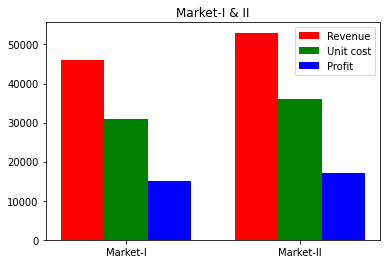
\includegraphics[width=\columnwidth]{solutions/su2021/45/FIGURE.png}
\caption{Revenue,Sales \& Profit Of Market-I \& II}
\label{matrix/2/45/fig:Profit}	
\end{figure}

  \item If A and B are square matrices of the same order such that AB=BA,then prove by indication that $AB^{n}=B^{n}A$.Further prove that $(AB)^{n}=A^{n}B^{n}$ for all $n \epsilon N$.\\
  Choose the correct answer in the following questions:\\
  \item If A=$\myvec{\alpha &\beta\\ \gamma &-\alpha}$ is such that $A^{2}=I$,then\\
  (A)$1+\alpha^{2}+\beta\gamma=0$ (B)$1-\alpha^{}2+\beta\gamma=0$\\
  (C)$1-\alpha^{2}-\beta\gamma=0$ (D)$1+\alpha^{2}-\beta\gamma=0$\\
\\
\solution
%
\begin{align}
    E(X) &= \frac{1}{\sqrt{2\pi}} \int_{-\infty}^{\infty} x e^{-\frac{x^2}{2}}dx\\
    &=0 \quad \brak{ \text{ odd function}}
\end{align}
\begin{align}
    E\brak{X^2}&= \frac{1}{\sqrt{2\pi}}\int_{-\infty}^{\infty} x^2
e^ {-\frac{x^2}{2}} dx \quad \brak{even function}\\
    &= \frac{2}{\sqrt{2\pi}} \int_{0}^{\infty} x^2 e^{-\frac{x^2}{2}} dx\\
    &= \frac{2}{\sqrt{2\pi}}\int_{0}^{\infty}\sqrt{2u}e^{-u} du \quad\brak{Let \frac{x^2}{2}= u}\\
    &= \frac{2}{\sqrt{\pi}} \int_{0}^{\infty} e^{-u} u^{\frac{3}{2}-1} du\\
    &= \frac{2}{\sqrt{\pi}} \Gamma\brak{{\frac{3}{2}}}\\
    &= \frac{1}{\sqrt{\pi}}\Gamma\brak{\frac{1}{2}} \\
    &= 1
\end{align}
where we have used the fact that
\begin{align}
\quad\because \Gamma(n)= (n-1)\Gamma(n-1); \Gamma\brak{\frac{1}{2}}=\sqrt{\pi}
\end{align}
%
Thus, the  variance is
\begin{align}
    \sigma^2 =  E\brak X^2 - E^2\brak X = 1
\end{align}

  \item If the matrix A is both symmetric and skew symmetric,then\\
  (A) A is a diagonal matrix \\
  (B) A is a zero matriz\\
  (C)A is a square matrix \\
  (D)None of these\\
  \\
\solution
If $\vec{A}$ is symmetric, then 
\begin{align}
\vec{A}^T =\vec{A}
\label{matrix/48/2.0.1}
\end{align}
If matrix A is skew symmetric, then
\begin{align}
\vec{A}^T = \vec{-A}
\label{matrix/48/2.0.2}
\end{align}
From  \eqref{matrix/48/2.0.1} and \eqref{matrix/48/2.0.2},
\begin{align}
\vec{A} &=\vec{-A}
\\
\implies 2\vec{A} &= 0
\\
\text{or, } \vec{A} &= 0
\end{align}
$\therefore $ $\vec{A}$ is zero matrix.


  \item If A is square matrix such that $A^{2}=A$,then $(I+A)^{3}-7A$ is equal to\\
  (A)A \\(B)I-A\\ (C)I\\ (D)3A
\\
\solution
%
\begin{align}
    E(X) &= \frac{1}{\sqrt{2\pi}} \int_{-\infty}^{\infty} x e^{-\frac{x^2}{2}}dx\\
    &=0 \quad \brak{ \text{ odd function}}
\end{align}
\begin{align}
    E\brak{X^2}&= \frac{1}{\sqrt{2\pi}}\int_{-\infty}^{\infty} x^2
e^ {-\frac{x^2}{2}} dx \quad \brak{even function}\\
    &= \frac{2}{\sqrt{2\pi}} \int_{0}^{\infty} x^2 e^{-\frac{x^2}{2}} dx\\
    &= \frac{2}{\sqrt{2\pi}}\int_{0}^{\infty}\sqrt{2u}e^{-u} du \quad\brak{Let \frac{x^2}{2}= u}\\
    &= \frac{2}{\sqrt{\pi}} \int_{0}^{\infty} e^{-u} u^{\frac{3}{2}-1} du\\
    &= \frac{2}{\sqrt{\pi}} \Gamma\brak{{\frac{3}{2}}}\\
    &= \frac{1}{\sqrt{\pi}}\Gamma\brak{\frac{1}{2}} \\
    &= 1
\end{align}
where we have used the fact that
\begin{align}
\quad\because \Gamma(n)= (n-1)\Gamma(n-1); \Gamma\brak{\frac{1}{2}}=\sqrt{\pi}
\end{align}
%
Thus, the  variance is
\begin{align}
    \sigma^2 =  E\brak X^2 - E^2\brak X = 1
\end{align}

\item Balance the following chemical equation.
\begin{align}
  \label{matrix/50/eq1}
NaOH + H_2SO_4 \xrightarrow{} Na_2SO_4  +  H_2O
\end{align}
\\
\solution
Let the balanced version of \eqref{matrix/50/eq1} be
\begin{align}
   x_{1}NaOH + x_{2}H_2SO_4 \xrightarrow{} 
   x_{3}Na_2SO_4 + x_{4}H_2O \label{matrix/50/eq2}
\end{align}
which results in the following equations:
\begin{align}
    (x_{1}-2x_{3}) Na= 0\\
    (x_{1}+4x_{2}-4x_{3}-x_{4}) O= 0\\
    (x_{1}+2x_{2}-2x_{4}) H=0\\
    (x_{2}-x_{3}) S= 0
\end{align}
which can be expressed as
\begin{align}
    x_{1}+ 0.x_{2}- 2x_{3}+ 0.x_{4} = 0\\
    x_{1}+ 4x_{2}- 4x_{3}- x_{4} = 0\\
    x_{1}+ 2x_{2}+ 0.x_{3}- 2x_{4} = 0\\
    0.x_{1}+ x_{2}- x_{3}+ 0.x_{4} = 0
\end{align}
resulting in the matrix equation
\begin{align}
    \myvec{1 & 0 & -2 & 0\\
           1 & 4 & -4 & -1\\
           1 & 2 & 0 & -2\\
           0 & 1 & -1 & 0}\vec{x}
           =\vec{0}    \label{matrix/50/eq3}
\end{align}
where,
\begin{align}
   \vec{x}= \myvec{x_{1}\\x_{2}\\x_{3}\\x_{4}}
\end{align}
\eqref{matrix/50/eq3} can be reduced as follows:
\begin{align}
    \myvec{1 & 0 & -2 & 0\\
           1 & 4 & -4 & -1\\
           1 & 2 & 0 & -2\\
           0 & 1 & -1 & 0}
    \xleftrightarrow[R_{3}\leftarrow R_3-R_{1}]{R_{2}\leftarrow R_2- R_1}
    \myvec{1 & 0 & -2 & 0\\
           0 & 4 & -2 & -1\\
           0 & 2 & 2 & -2\\
           0 & 1 & -1 & 0}\\
    \xleftrightarrow{R_2 \leftarrow \frac{R_2}{4}}
    \myvec{1 & 0 & -2 & 0\\
          0 & 1 & -\frac{1}{2} & -\frac{1}{4}\\
          0 & 2 & 2 & -2\\
          0 & 1 & -1 & 0}\\
    \xleftrightarrow[R_4 \leftarrow R_4 - R_2]{R_3 \leftarrow R_3 - 2R_2}
    \myvec{1 & 0 & -2 & 0\\
           0 & 1 & -\frac{1}{2} & -\frac{1}{4}\\
           0 & 0 & 3 & -\frac{3}{2}\\
           0 & 0 & -\frac{1}{2} & \frac{1}{4}}\\
    \xleftrightarrow{R_3 \leftarrow \frac{R_3}{3}}
    \myvec{1 & 0 & -2 & 0\\
           0 & 1 & -\frac{1}{2} & -\frac{1}{4}\\
           0 & 0 & 1 & -\frac{1}{2}\\
           0 & 0 & -\frac{1}{2} & \frac{1}{4}}\\
    \xleftrightarrow[R_{4}\leftarrow R_4+\frac{R_3}{2}]{R_{2}\leftarrow R_2+ \frac{R_3}{2}}
    \myvec{1 & 0 & -2 & 0\\
           0 & 1 & 0 & -\frac{1}{2}\\
           0 & 0 & 1 & -\frac{1}{2}\\
           0 & 0 & 0 & 0}\\
    \xleftrightarrow{R_1 \leftarrow R_1+2R_3}
    \myvec{1 & 0 & 0 & -1\\
           0 & 1 & 0 & -\frac{1}{2}\\
           0 & 0 & 1 & -\frac{1}{2}\\
           0 & 0 & 0 & 0}
\end{align}
Thus,
\begin{align}
    x_1=x_4, x_2= \frac{1}{2}x_4, x_3=\frac{1}{2}x_4\\
    \implies \quad\vec{x}= x_4\myvec{1\\ \frac{1}{2}\\ \frac{1}{2}\\1} 
\end{align} 
by substituting $x_4= 2$
\begin{align}
    \vec{x}=\myvec{2\\1\\1\\2}
\end{align}
Hence, \eqref{matrix/50/eq2} finally becomes
\hfill\break
%\vspace{5mm}  finally becomes
\begin{align}
    2 NaOH + H_2SO_4 \xrightarrow{} 
    Na_2SO_4 + 2 H_2O
\end{align}

\item Balance the following chemical equation
\begin{align}\label{1}
    BaCl_2 + H_2SO_4 \xrightarrow{} BaSO_4 + HCl
\end{align}
    \item If A=\myvec{1 &2 &3\\2 &3 &1} and B=\myvec{3 &-1 &3\\-1 &0 &2}, then find 2A-B.\\
    \item If A=\myvec{8 &0\\4 &-2\\3 &6} and B=\myvec{2 &-2\\4 &2\\-5 &1}, then find the matrix X, such that 2A+3X=5B.\\
    \item Find X and Y, if X+Y=\myvec{5 &2\\0 &9} and \\X-Y=\myvec{3 &6\\0 &-1}.\\
    \item Find the values of x and y from the following equation:\\
    2\myvec{x &5\\7 &y-3} + \myvec{3 &-4\\1 &2} = \myvec{7 &6\\15 &14}\\
     
    

\item     Two farmers Ramkishan and Gurcharan Singh cultivate only three varieties of rice namely Basmati, Permal and Naura. The sale (in Rupees) of these varieties of rice by both the farmers in the month of September and October are given by the following matrices $\vec{A}$ and $\vec{B}$ .

\begin{center}
September Sales(in Rupees)
\end{center}
\begin{align}
    \vec{A}=
    \begin{blockarray}{cccc}
    \text{Basmati} & \text{Permal} & \text{Naura} \\
    \begin{block}{(ccc)(c)}
    10000 & 20000 & 30000 & \text{Ramkishan}\\
    50000 & 30000 & 10000 & \text{Gurucharan} \\
    \end{block}
    \end{blockarray}
\end{align}

\begin{center}
October Sales(in Rupees)
\end{center}
\begin{align}
    \vec{B} =
    \begin{blockarray}{cccc}
    \text{Basmati} & \text{Permal} & \text{Naura} \\
    \begin{block}{(ccc)(c)}
    5000 & 10000 & 6000 & \text{Ramkishan}\\
    20000 & 10000 & 10000 & \text{Gurucharan} \\
    \end{block}
    \end{blockarray}
\end{align}

\begin{enumerate}
    \item Find the combined sales in September and October for each farmer in each variety.
    \item Find the decrease in sales from September to October.
    \item If both farmers receive 2\% profit on gross sales, compute the profit for each farmer and for each variety sold in October.
\end{enumerate}
%
\solution

The given system of inequality can be written in matrix form as
\begin{align}
    \myvec{-1 & -2  \\ -1 & 1 \\ 1 & 1\\ 1 & 0 \\ 0 & 1}\vec{x} \succeq \myvec{-10\\0\\1\\0\\0}
\end{align}
which can be further simplified into 
\begin{align}
    \myvec{-1 & -2 \\ 1 & 0 \\ 0&1}\vec{x} \succeq \myvec{-10\\\frac{-1}{2}\\\frac{-1}{2}}
\end{align}
Let the surplus vector be
\begin{align}
    \vec{u} &= \myvec{u_1\\u_2} \succeq 0
\end{align}
\begin{enumerate}
    \item 
    \begin{align}
        \myvec{-1 & -2 \\ 1 & 0}\vec{x} &\succeq \myvec{-10 \\ \frac{-1}{2}}
        \\
        \implies  \myvec{-1 & -2 \\ 1 & 0}\vec{x} &= \myvec{-10 \\ \frac{-1}{2}} + \vec{u}
    \end{align}
    resulting in 
    \begin{align}
        \vec{x} &= \myvec{-1 & -2 \\ 1 & 0}^{-1}\myvec{-10 \\\frac{-1}{2}} + \myvec{-1 & -2 \\ 1 & 0}^{-1}\vec{u}
        \\
        \implies \vec{x} &= \myvec{\frac{1}{2} \\ \frac{19}{4}} + \myvec{0&1\\ \frac{-1}{2}&\frac{-1}{2}}\vec{u}   \label{ineq/58/eq1}
    \end{align}
    \item 
    \begin{align}
        \myvec{-1& -2 \\ 0 & 1}\vec{x} &\succeq \myvec{-10 \\ \frac{-1}{2}}
        \\
        \implies  \myvec{-1& -2 \\ 0 & 1}\vec{x} &= \myvec{-10 \\ \frac{-1}{2}} + \vec{u}
    \end{align}
    resulting in 
    \begin{align}
        \vec{x} &= \myvec{-1& -2 \\ 0 & 1}^{-1}\myvec{-10 \\ \frac{-1}{2}} + \myvec{-1& -2 \\ 0 & 1}^{-1}\vec{u}
        \\
        \implies \vec{x} &= \myvec{9\\\frac{1}{2}} + \myvec{-1& -2 \\ 0 & 1}\vec{u} \label{ineq/58/eq2}
    \end{align}
\end{enumerate}
Now,solution region which is common to regions of eq. \eqref{ineq/58/eq1} and eq. \eqref{ineq/58/eq2},is given by
\begin{align}
    \boxed{\vec{x} = \myvec{\frac{1}{2}\\\frac{1}{2}}+\myvec{0&1\\\frac{-1}{2}&1}\vec{u}}
\end{align}
%
\begin{figure}[!ht]
\centering
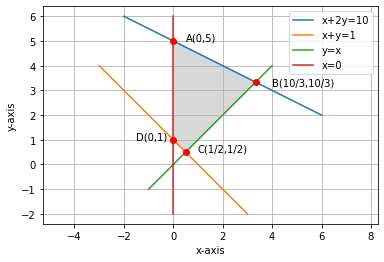
\includegraphics[width=\columnwidth]{solutions/su2021/2/58/Figures/Figure_2.58.png}
\caption{Graphical Solution}
\label{ineq/58/fig:fig1}	
\end{figure}

\begin{figure}[!ht]
\centering
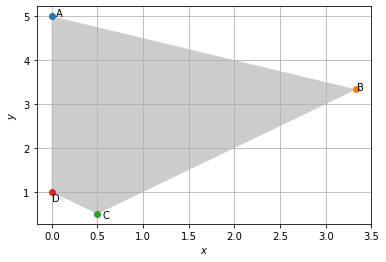
\includegraphics[width=\columnwidth]{solutions/su2021/2/58/Figures/2.58(2).png}
\caption{Magnified Solution region}
\label{ineq/58/fig:fig2}	
\end{figure}


   
    \item  Find AB, if A=\myvec{6 &9\\2 &3} and B=\myvec{2 &6 &0\\7 &9 &8}.\\
    \item  If A=\myvec{1 &-2 &3\\-4 &2 &5\\} and B=\myvec{2 &3\\4 &5\\2 &1}, then find AB,BA.Show that AB$\neq$BA

   
     \item If A=\myvec{1 &0 \\0 &-1} and  B=\myvec{0 &1\\1 &0}, then find AB,BA. Show that AB$\neq$BA\\
     
   
    \item Find AB, if A=\myvec{0 &-1\\0 &2} and B=\myvec{3 &5\\0 &0}\\
     
   
    \item If A=\myvec{1 &1 &-1\\2 &0 &3\\3 &-1 &2}, B=\myvec{1 &3\\0 &2\\-1 &4} and C=\myvec{1 &2 &3 &-4\\2 &0 &-2 &1}, find\\A(BC),(AB)C and show that (AB)C=A(BC) \\   
    
     \item If A=\myvec{0 &6 &7\\-6 &0 &8\\7 &-8 &0}, B=\myvec{0 &1 &1\\1 &0 &2\\1 &2 &0},C=\myvec{2\\-2\\3}\\Calculate AC,BC and (A+B)C=AC+BC\\

    \item If A=$\myvec{1 &2 &3\\3 &-2 &1\\4 &2 &1}$,then show that $A^3-23A-40I=0$
  \\  
  \solution
  Given that $\vec{A}$ =$\myvec{1&2&3\\3&-2&1\\4&2&1}$.
\begin{enumerate}
\item \textbf{The Characteristic equation} is given by:
\begin{align}
  \implies  \abs{\vec{A}-\lambda\vec{I}}&=0
    \\
    \implies \mydet{1-\lambda&2&3\\3&-2-\lambda&1\\4&2&1-\lambda}&=0
    \end{align}
\begin{multline}
   \implies\brak{1-\lambda}\brak{\brak{-2-\lambda}\brak{1-\lambda}-2}
   \\
   -2\brak{3\brak{1-\lambda}-4}+3\brak{6+4\brak{2+\lambda}}=0
\end{multline}
\begin{align}
 \implies   \lambda^3-23\lambda-40=0
\end{align}
The above equation is similar to equation to be proved.
\item According to \textbf{Cayley-Hamilton Theorem:} 
\\
Every square matrix satisfies its own
\\\textbf{characteristic equation}.
\begin{align}
\therefore    \vec{A}^3-23\vec{A}-40\vec{I}=0
\end{align}
Hence Proved.
\end{enumerate}
    
    
\item In a legislative assembly election, a political
group hired a public relations firm to promote
its candidate in three ways: telephone, house
calls, and letters. The cost per contact (in paise)
is given in matrix $\vec{A}$ as
\begin{center}
Cost per Contact(in Paise)
\end{center}
\begin{align}
    \vec{A}=
    \begin{blockarray}{cc}
    \text{cost}\\
    \begin{block}{(c)(c)}
    40 &\text{Telephone}\\
    100&\text{Housecall} \\
    50&\text{Letter}\\
    \end{block}
    \end{blockarray}
\end{align}
The number of contacts of each type made in
two cities X and Y is given by matrix $\vec{B}$
\begin{align}
    \vec{B} =
    \begin{blockarray}{cccc}
    \text{Telephone} & \text{Housecall} & \text{Letter} \\
    \begin{block}{(ccc)(c)}
    1000 & 500 & 5000 & \text{X}\\
    3000 & 1000 & 10000 & \text{Y} \\
    \end{block}
    \end{blockarray}
\end{align}
Find the total
amount spent by the group in the two cities
X and Y
%
\solution

The total amount spent is given by=

    \begin{multline}
    \vec{B}\vec{A}\\
    =\myvec{1000&500&5000\\3000&1000&10000}\myvec{40\\100\\50}\\
    =\myvec{40000+50000+250000\\120000+100000+500000}\\
    \begin{blockarray}{cc}
    \text{TotalCost} \\
    \begin{block}{(c)(c)}
    340000&\text{X}\\
    720000&\text{Y}\\
    \end{block}
    \end{blockarray}
    \end{multline}
$\therefore$ the total amount spent in city X and city Y is 3400 and 7200 Rupees respectively.  See Fig. \ref{matrix/64fig:Profit}	
%
\begin{figure}[!ht]
\centering
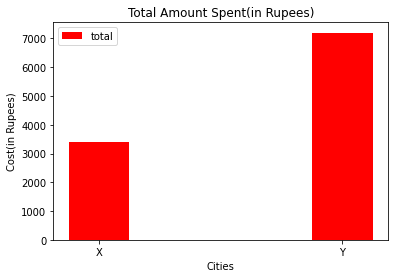
\includegraphics[width=\columnwidth]{solutions/su2021/64/figure8.png}
\caption{Total Amount Spent by the group in cities X and Y}
\label{matrix/64fig:Profit}	
\end{figure}


\item If A=$\myvec{3 &\sqrt{3} &2\\4 &2 &0}$ and B=$\myvec{2 &-1 &2\\1 &2 &4}$, verify that\\
(i) $(A^{'})^{'}=A$\\ (ii)$(A+B)^{'}=A^{'}+B^{'}$,\\ (iii) $(kB)^{'}=kB^{'}$,where k is any constant.\\
\item If A=$\myvec{-2\\4 \\5}$,B=$\myvec{1 &3 &-6}$, verify that $(AB)^{'}=B^{'}A^{'}$\\
\item Express the matrix B=$\myvec{2 &-2 &-4\\-1 &3 &4\\1 &-2 &-3}$ as the sum of a symmetric and a skew symmetric matrix.\\
\solution
  We obtain the vertices of the rhombus as follows
\begin{align}
\vec{A} = \myvec{-3\\0},
\vec{B} = \myvec{0\\-3.5},
\vec{C} = \myvec{3\\0},
\vec{D} = \myvec{0\\3.5}
\end{align}
which are plotted in Fig. \ref{quad/45/fig:Rhombus ABCD}.
%
\begin{figure}[ht!]
\centering
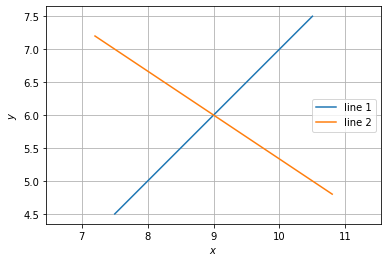
\includegraphics[width=\columnwidth]{solutions/quad/45/figure2.png}
\caption{Rhombus ABCD}
\label{quad/45/fig:Rhombus ABCD}
\end{figure}

  
\item By using elementary operations,find the inverse of the matrix\\
A=$\myvec{1 &2\\2 &-1}$.\\
\item Obtain the inverse of the following matrix using elementary operations\\
A=$\myvec{0 &1 &2\\1 &2 &3\\3 &1 &1}$.\\
\solution
  \begin{enumerate}
    \item Given that
    \begin{align}
    \vec{A}& =\myvec {0 & 1 & 2\\1 & 2 & 3\\3 & 1 & 1}
    \end{align}
     The augmented matrix $[A | I]$ is as given below:- 
    \begin{align}
    \myvec{0 & 1 & 2 & \vrule & 1 & 0 & 0\\1 & 2 & 3 & \vrule & 0 & 1 & 0\\3 & 1 & 1 & \vrule & 0 & 0 & 1}
    \end{align}
    We apply the elementary row operations on $[A | I]$ as follows :-
    \begin{align}
    [A | I] = \myvec{0 & 1 & 2 & \vrule & 1 & 0 & 0\\1 & 2 & 3 & \vrule & 0 & 1 & 0\\3 & 1 & 1 & \vrule & 0 & 0 & 1}
    \\
    \xleftrightarrow{R_1\leftrightarrow R_2}   
    \myvec{1 & 2 & 3 & \vrule & 0 & 1 & 0\\0 & 1 & 2 & \vrule & 1 & 0 & 0\\3 & 1 & 1 & \vrule & 0 & 0 & 1}
    \\
    \xleftrightarrow{R_3\leftarrow R_3-3R_1}   
    \myvec{1 & 2 & 3 & \vrule & 0 & 1 & 0\\0 & 1 & 2 & \vrule & 1 & 0 & 0\\0 & -5 & -8 & \vrule & 0 & -3 & 1}
    \\
    \xleftrightarrow{R_1\leftarrow R_1-2R_2}  
    \myvec{1 & 0 & -1 & \vrule & -2 & 1 & 0\\0 & 1 & 2 & \vrule & 1 & 0 & 0\\0 & -5 & -8 & \vrule & 0 & -3 & 1}
    \\
    \xleftrightarrow{R_3\leftarrow R_3+5R_2}  
    \myvec{1 & 0 & -1 & \vrule & -2 & 1 & 0\\0 & 1 & 2 & \vrule & 1 & 0 & 0\\0 & 0 & 2 & \vrule & 5 & -3 & 1}
    \\
    \xleftrightarrow{R_3\leftarrow R_3/2}
    \myvec{1 & 0 & -1 & \vrule & -2 & 1 & 0\\ 0 & 1 & 2 & \vrule & 1 & 0 & 0\\0 & 0 & 1 &\vrule &\frac{5}{2} &\frac{-3}{2} &\frac{1}{2}}
    \\
    \xleftrightarrow{R_1\leftarrow R_1+R_3}
    \myvec{1 & 0 & 0 & \vrule & \frac{1}{2} & \frac{-1}{2} & \frac{1}{2}\\ 0 & 1 & 2 & \vrule & 1 & 0 & 0\\0 & 0 & 1 &\vrule &\frac{5}{2} &\frac{-3}{2} &\frac{1}{2}}
    \\
    \xleftrightarrow{R_2\leftarrow R_2-2R_3}
    \myvec{1 & 0 & 0 & \vrule & \frac{1}{2} & \frac{-1}{2} & \frac{1}{2}\\ 0 & 1 & 0 & \vrule & -4 & 3 & -1\\0 & 0 & 1 &\vrule &\frac{5}{2} &\frac{-3}{2} &\frac{1}{2}}
    \end{align}
    By performing elementary transformations on augmented matrix$ [A | I]$ , we obtained the augmented matrix in the form $ [I | A]$. 
    Hence we can conclude that the matrix A is invertible and inverse of the matrix is:-
    \begin{align}
    \therefore\vec{A^{-1}}=\myvec { \frac{1}{2} & \frac{-1}{2} & \frac{1}{2} \\  -4 & 3 & -1\\ \frac{5}{2} &\frac{-3}{2} &\frac{1}{2}}
    \end{align}
    \item QR decomposition of  \myvec{0  & 1 & 3 \\ 1 & 2 & 3 \\ 2 & 3 & 1}
    \\
     Let us use the Gram-schmidt approach to obtain QR decomposition of$ \vec{A}$. Consider rows vectors say $\vec{a_1}$,$\vec{a_2}$ and $\vec{a_3}$ of $\vec{A}$  which is given by
    \begin{align}
    \vec{a_1}=\myvec{0 & 1 & 2}\label{matrix/69/eq1}\\
    \vec{a_2}=\myvec{1 & 2 & 3}\label{matrix/69/eq2}\\
    \vec{a_3}=\myvec{3 & 1 & 1}\label{matrix/69/eq3}
    \end{align}
    we can express these as 
    \begin{align}
    \vec{u_1}&=\vec{a_1}=\myvec{0 & 1 & 2}\label{matrix/69/eq4}\\
    \vec{e_1}&=\frac{\vec{u_1}}{\norm{\vec{u_1}}}\\
    \vec{e_1}&=\frac{\myvec{0 & 1 & 2}}{\sqrt{0+1+4}}\\
    \vec{e_1}&=\myvec{0 & \frac{1}{\sqrt{5}} & \frac{2}{\sqrt{5}}}\\
    \vec{u_2}&=\vec{a_2}-(\vec{a_2}\vec{e_1})\vec{e_1}\\
    &=\myvec{1 & 2 & 3}-(\myvec{1 & 2 & 3}\myvec{0 & \frac{1}{\sqrt{5}} & \frac{2}{\sqrt{5}}})\myvec{0 & \frac{1}{\sqrt{5}} &  \frac{2}{\sqrt{5}}}\\
    &=\myvec{1 & \frac{2}{5} & \frac{-1}{5}}\\
    \vec{e_2}&=\frac{\vec{u_2}}{\norm{\vec{u_2}}}=\frac{\myvec{1 & \frac{2}{5} & \frac{-1}{5}}}{\sqrt{1+\frac{4}{25}+\frac{1}{25}}}\\
    \vec{e_2}&=\myvec{\frac{5}{\sqrt{30}} & \frac{2}{\sqrt{30}} &\frac{-1}{\sqrt{30}}}\\
    \vec{u_3}&=\vec{a_3}-(\vec{a_3}\vec{e_1})\vec{e_1}-(\vec{a_3}\vec{e_2})\vec{e_2}
    \\
    \vec{u_3}&=\myvec{\frac{1}{3} & \frac{-2}{3} &\frac{1}{3}}\\
    \vec{e_3}&=\frac{\vec{u_3}}{\norm{\vec{u_3}}}\\
    &=\frac{\myvec{\frac{1}{3} & \frac{-2}{3} & \frac{1}{4}}}{\sqrt{\frac{1}{9}+\frac{4}{9}+\frac{1}{9}}}\\
    \vec{e_3}&=\myvec{\frac{1}{\sqrt{6}} & \frac{-2}{\sqrt{6}} &\frac{1}{\sqrt{6}}}
    \end{align}
    Thus,
    \begin{align}
     \vec{Q}&=(e_1|e_2|----|e_n)\\
     &=\myvec{0 & \frac{5}{\sqrt{30}} & \frac{1}{\sqrt{6}}\\\frac{1}{\sqrt{5}} & \frac{2}{\sqrt{30}} & \frac{-2}{\sqrt{6}}\\\frac{2}{\sqrt{5}} & \frac{-1}{\sqrt{30}} & \frac{1}{\sqrt{6}}}\label{matrix/69/eq5}      
    \end{align}
    Then
    \begin{align}
      \vec{R}&=\myvec{a_1e_1 & a_2e_1 & a_3e_1\\ 0 & a_2e_2 & a_3e_2\\0 & 0 & a_3e_3}\\
      &=\myvec{\frac{5}{\sqrt{5}} & \frac{8}{\sqrt{5}} & \frac{3}{\sqrt{5}}\\0 &  \frac{6}{\sqrt{30}} & \frac{16}{\sqrt{30}}\\0 & 0 & \frac{2}{\sqrt{6}}}\label{matrix/69/eq6} 
      \end{align}
    From equations \eqref{matrix/69/eq5} and \eqref{matrix/69/eq6} the obtained $\vec{Q} \vec{R}$ Decomposition is
    \begin{align}
     \myvec{0  & 1 & 3 \\ 1 & 2 & 3 \\ 2 & 3 & 1}&= \myvec{0 & \frac{5}{\sqrt{30}} & \frac{1}{\sqrt{6}}\\\frac{1}{\sqrt{5}} & \frac{2}{\sqrt{30}} & \frac{-2}{\sqrt{6}}\\\frac{2}{\sqrt{5}} & \frac{-1}{\sqrt{30}} & \frac{1}{\sqrt{6}}}\myvec{\frac{5}{\sqrt{5}} & \frac{8}{\sqrt{5}} & \frac{3}{\sqrt{5}}\\0 &  \frac{6}{\sqrt{30}} & \frac{16}{\sqrt{30}}\\0 & 0 & \frac{2}{\sqrt{6}}} 
    \end{align}
    \end{enumerate}

\item Find P$^{-1}$, if it exists, given \\
P=$\myvec{10 &-2\\-5 &1}$.\\
\solution
Using row reduction, 
%
\begin{align}
\myvec{10 & -2 \\-5 & 1}
\xleftrightarrow {R_2 \leftarrow R_2+\frac{R_1}{2}}\myvec{10& -2& \\0 & 0}
\end{align} 
Hence,  $\vec {P}^{-1} $ does not exist.
\item If A=$\myvec{\cos\theta &\sin\theta\\ \-sin\theta &\cos\theta}$,\\then prove that $A^{n}=\myvec{\cos\theta &\sin n\theta\\\-sin n\theta &\cos n\theta}$, n $\in$ N.\\
\item If A and B are symmetric matrices of the same order, then show that AB is symmetric if and only if A and B commute,that AB = BA.\\
\item Let A=$\myvec{2 &-1\\3 &4}$, B=$\myvec{5 &2\\7 &4}$, C=$\myvec{2 &5\\3 &8}$. Find a matrix D such that CD-AB=0. 
\item Find the values of a,b,c and d from the equations: \myvec{a-b &2a+c\\2a-b &3c+d} = \myvec{-1 &5\\0 &13}
\item Show that\\
(i)$\myvec{5 &-1\\6 &7}\myvec{2 &1\\3 &4}\neq\myvec{2 &1\\3 &4}\myvec{5 &-1\\6 &7}$
\\
(ii)$\myvec{1 &2 &3\\0 &1 &0\\1 &1 &0}\myvec{-1 &1 &0\\0 &-1 &1\\2 &3 &4}\neq \myvec{-1 &1 &0\\0 &-1 &1\\2 &3 &4}\myvec{1 &2 &3\\0 &1 &0\\1 &1 &0}$\\
\item If A=\myvec{3 &-2\\4 &-2} and I=\myvec{1 &0\\0 &1},find k\\
 so that $A^2=kA-2I$\\
  \item Find the matrix X so that\\ X\myvec{1 &2 &3\\4 &5 &6}=\myvec{-7 &-8 &-9\\2 &4 &6}\\
\item (i) $\begin{vmatrix}a-b-c& 2a& 2a \\ 2b& b-c-a& 2b \\ 2c& 2c& c-a-b\end{vmatrix}$= $(a+b+c)^3$\\
(ii) $\begin{vmatrix}x+y+2z&x&y \\ z&y+z+2x&y \\ z&x&z+x+2y\end{vmatrix}$=$2(x+y+z)^3$
\item $\begin{vmatrix}1&x&x^2 \\ x^2&1&x \\ x&x^2&1\end{vmatrix}$=$(1-x^3)^2$ 
\item $\begin{vmatrix}1+a^2-b^2&2ab&-2b \\ 2ab&1-a^2+b^2&2a \\ 2b&-2a&1-a^2-b^2\end{vmatrix}$=$(1+a^2+b^2)^3$
\item Let 
A=$\begin{bmatrix}
1&\sin\theta&1 \\ -\sin\theta&1&\sin\theta \\ -1&-\sin\theta&1
\end{bmatrix},$ 
where $0\leq \theta \leq 2\Pi.$ Then
\begin{enumerate}
\item Det(A)=0
\item Det(A)$\in(2,\infty)$
\item Det(A)$\in (2,4)$
\item Det(A)$\in [2,4]$
\end{enumerate}
\item $\begin{vmatrix}
1&1+p&1+p+q \\ 2&3+2p&4+3p+2q \\ 3&6+3p&10+6p+3q
\end{vmatrix}$=1\\
\item $\begin{vmatrix}\sin\alpha&\cos\alpha&\cos(\alpha+\delta) \\ \sin\beta&\cos\beta&\cos(\beta+\delta) \\ \sin\gamma&\cos\gamma&\cos(\gamma+\delta)\end{vmatrix}$=0\\
\item Solve the system of equations \\$\frac{2}{x}+\frac{3}{y}+\frac{10}{z}=4$\\$\frac{4}{x}-\frac{6}{y}+\frac{5}{z}=1$\\$\frac{6}{x}+\frac{9}{y}-\frac{20}{z}=2$\\
\item If a,b,c are in A.P, then the determinant\\
 $\begin{vmatrix}
x+2&x+3&x+2a \\ x+3&x+4&x+2b \\x+4&x+5&x+2c
\end{vmatrix}$ is 
\begin{enumerate}
\item 0
\item 1
\item x
\item 2x
\end{enumerate}
\item If x,y,z are nonzero real numbers, then the inverse of matrix 
A=$\begin{bmatrix}
x&0&0 \\ 0&y&0 \\ 0&0&z
\end{bmatrix}$ is 
\begin{enumerate}
\item $\begin{bmatrix} x^{-1}&0&0 \\ 0&y^{-1}&0 \\ 0&0&z^{-1} \end{bmatrix}$ 
\item $xyz\begin{bmatrix} x^{-1}&0&0 \\ 0&y^{-1}&0 \\ 0&0&z^{-1} \end{bmatrix}$ 
\item $\frac{1}{xyz}\begin{bmatrix} x&0&0 \\ 0&y&0 \\ 0&0&z \end{bmatrix}$ 
\item $\frac{1}{xyz}\begin{bmatrix} 1&0&0 \\ 0&1&0 \\ 0&0&1 \end{bmatrix}$ 
\end{enumerate}
\textbf{Examine the consistency of the system of given Equations.}
\item 
$\begin{alignedat}[t]{2}
x+2y&=2 
\\
2x+3y&=3 
\end{alignedat}$
\item $\begin{alignedat}[t]{2}
2x-y&=5 
\\
x+y&=4 
\end{alignedat}$
\item Evaluate the determinant
$\begin{vmatrix}0&a&-b\\-a&0&-c\\b&c&0\end{vmatrix}=0$
\\
Find the inverse and QR decomposition of the following.
  \item \myvec{2 &1\\1 &1}\\
  \item\myvec{1 &3\\2 &7}\\
  \item\myvec{2 &3\\5 &7}\\
  \item\myvec{2 &1\\7 &4}\\
  \item \myvec{2 &5\\1 &3}\\
  \item \myvec{3 &1\\5 &2}\\
  \item \myvec{4 &5\\3 &4}\\
  \item \myvec{3 &10\\2 &7}\\
  \item \myvec{3 &-1\\-4 &2}\\
  \item \myvec{2 &-6\\1 &-2}\\
  \item \myvec{6 &-3\\-2 &1}\\
  \item \myvec{2 &-3\\-1 &2}\\
  \item \myvec{2 &1\\4 &2}\\
\item Find the QR decomposition of 
\begin{align}
\vec{A}=\myvec{8&5\\3&2} \label{eq:solutions/decomp/2/29/eq:1}
\end{align}
%%
%
\item Find the QR decomposition of 
\begin{align}
\vec{A}=\myvec{2&5\\1&4} \label{eq:solutions/decomp/2/30/1}
\end{align}

%    \end{document}    

